\documentclass[conference]{IEEEtran}
\usepackage{times}
\usepackage[numbers]{natbib}
\usepackage{multicol}
\usepackage[bookmarks=true]{hyperref}
\usepackage{graphicx}
\usepackage{amsmath}
\usepackage{amssymb}
\usepackage{tikz}
\usetikzlibrary{positioning,fit,arrows.meta,shapes.geometric}

\hypersetup{
    pdfauthor={Anonymous},
    pdftitle={Modular Language-Guided Robotic Manipulation: Integrating NL-DSL Grounding and Closed-Loop Visual Feedback},
    pdfsubject={Robotics},
    pdfkeywords={Vision-Language-Action Models, Robot Manipulation, Imitation Learning, Generalization}
}

\begin{document} 

\title{Modular Language-Guided Robotic Manipulation: \\Integrating NL-DSL Grounding and Closed-Loop Visual Feedback}

\author{Yingjun Lan, Jinhao Zhang, Zhengxiang Liu}

\maketitle

\begin{abstract}
Traditional imitation learning (e.g., Robomimic \cite{robomimic2021}) relies on open-loop visual-to-action mappings, lacking structural semantic understanding and robustness against perturbations. We propose extending the Robomimic pick-up task with two innovations: (1) an NL+DSL (Natural Language to Domain-Specific Language) paradigm for precise command parsing, and (2) closed-loop visual feedback for dynamic trajectory regulation. Our system uses a vision-language-action (VLA) model to ground DSL constraints into target objects and 3D grasp poses, which are fed to a low-level policy. By incorporating real-time visual feedback, the policy adjusts actions dynamically. Evaluated on out-of-distribution scenes, we expect our framework to significantly outperform open-loop, pure-NL baselines in generalization and error recovery.
\end{abstract}

\section{Introduction and Motivation}
\label{sec:intro} 

Recent vision-language-action systems have shown strong potential for robotic control, but robustness in out-of-distribution scenes remains a key challenge \cite{robomonkey2025}. At the same time, task-level progress awareness and recovery are increasingly important for long-horizon manipulation \cite{sprvla2026}.

This project is proposed as a \textbf{research project} that builds upon the ``General robot pick-up skills learning'' idea (2.3) and incorporates elements of ``Language-guided motion generation'' (2.5) from the idea pool. To improve upon pure open-loop execution and ambiguous natural language parsing, we introduce two key innovations: (1) adopting a Natural Language + symbolic abstraction paradigm inspired by recent LLM-guided planning work \cite{plahx2025}, and (2) incorporating a closed-loop feedback regulation mechanism during execution, motivated by progress-aware VLA control \cite{sprvla2026}. We aim to answer the following research question: \emph{Can a modular integration of a pre-trained VLA, utilizing symbolic language grounding and robust visual feedback, improve the generalization of robotic pick-up tasks to novel visual and semantic variations?} By addressing this question, we seek to demonstrate a practical and computationally feasible method for enhancing existing manipulation frameworks with formal grounding and error recovery capabilities.

\section{Literature Review}
\label{sec:literature}

\paragraph{VLA Robustness and Test-Time Scaling}
Recent work shows that VLA robustness can be improved significantly at inference time by sampling and verification instead of single-pass action generation \cite{robomonkey2025}. This suggests a practical path for course-scale systems: keep the base policy lightweight and improve reliability through test-time decision mechanisms.

\paragraph{Modular Planning and Progress-Aware Control}
Recent LLM-guided planning work demonstrates that compact symbolic abstractions can improve task planning efficiency and reliability compared to verbose formulations \cite{plahx2025}. In parallel, progress-aware VLA control with explicit sub-goals and rewind-style recovery improves robustness in long-horizon manipulation \cite{sprvla2026}. Beyond manipulation, large-scale motion control studies also support the value of modular, representation-driven control pipelines \cite{moconvq2023}.

\section{Technical Plan}
\label{sec:technical}

\subsection{System Overview}
The proposed system consists of four primary modules (Fig.~\ref{fig:architecture}):
\begin{enumerate}
    \item \textbf{NL+Symbolic Parsing Module \cite{plahx2025}:} A lightweight LLM translates natural language queries into a compact symbolic task representation with clear action constraints.
    \item \textbf{Semantic Perception Module:} A vision-language grounder uses the DSL and RGB observation to localize targets (e.g., bounding boxes).
    \item \textbf{Grasp Planning Module:} Computes a 6-DoF target grasp pose to serve as an execution sub-goal.
    \item \textbf{Closed-Loop Execution \& Feedback Module \cite{sprvla2026}:} A Robomimic policy translates the sub-goal to joint actions, while continuous visual feedback and progress monitoring correct runtime deviations.
\end{enumerate}

\begin{figure}[ht]
\centering
\scriptsize
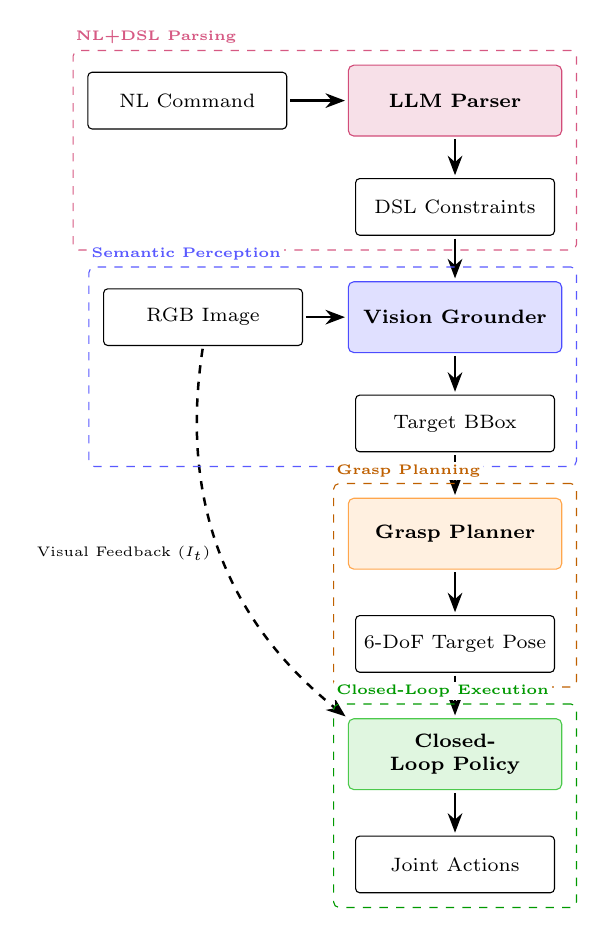
\begin{tikzpicture}[
    box/.style={rectangle, draw, rounded corners=1.5pt, minimum width=2.5cm, minimum height=0.72cm, text width=2.35cm, align=center, font=\scriptsize, inner sep=2.5pt},
    module/.style={rectangle, draw=#1!70, fill=#1!12, rounded corners=2pt, minimum width=2.7cm, minimum height=0.9cm, text width=2.5cm, align=center, font=\scriptsize\bfseries, inner sep=3pt},
    arrow/.style={->, >=Stealth, line width=0.9pt, shorten >=1pt, shorten <=1pt}
]

% Inputs (left / right) and main vertical pipeline
\node[box] (img) at (-3.2,-2.65) {RGB Image};
\node[box] (lang) at (-3.4,0.1) {NL Command};

\node[module=purple] (llm) at (0,0.1) {LLM Parser};
\node[box] (dsl) at (0,-1.25) {DSL Constraints};
\node[module=blue] (vla) at (0,-2.65) {Vision Grounder};
\node[box] (bbox) at (0,-4.0) {Target BBox};
\node[module=orange] (grasp) at (0,-5.4) {Grasp Planner};
\node[box] (pose) at (0,-6.8) {6-DoF Target Pose};
\node[module=green!70!black] (policy) at (0,-8.2) {Closed-Loop Policy};
\node[box] (action) at (0,-9.6) {Joint Actions};

% Arrows
\draw[arrow] (lang.east) -- (llm.west);
\draw[arrow] (llm.south) -- (dsl.north);
\draw[arrow] (dsl.south) -- (vla.north);
\draw[arrow] (img.east) -- (vla.west);
\draw[arrow] (vla.south) -- (bbox.north);
\draw[arrow] (bbox.south) -- (grasp.north);
\draw[arrow] (grasp.south) -- (pose.north);
\draw[arrow] (pose.south) -- (policy.north);
\draw[arrow] (policy.south) -- (action.north);
\draw[arrow, dashed, bend right=30] (img.south) to node[left, font=\tiny] {Visual Feedback ($I_t$)} (policy.north west);

% Dashed stage grouping
\node[draw=purple!65, dashed, rounded corners=2pt, inner sep=0.18cm, fit=(lang) (llm) (dsl)] (nl) {};
\node[anchor=south west, font=\tiny\bfseries, text=purple!65, fill=white, inner sep=1pt] at ([yshift=1pt]nl.north west) {NL+DSL Parsing};

\node[draw=blue!65, dashed, rounded corners=2pt, inner sep=0.18cm, fit=(img) (vla) (bbox)] (perception) {};
\node[anchor=south west, font=\tiny\bfseries, text=blue!65, fill=white, inner sep=1pt] at ([yshift=1pt]perception.north west) {Semantic Perception};

\node[draw=orange!75!black, dashed, rounded corners=2pt, inner sep=0.18cm, fit=(grasp) (pose)] (planning) {};
\node[anchor=south west, font=\tiny\bfseries, text=orange!75!black, fill=white, inner sep=1pt] at ([yshift=1pt]planning.north west) {Grasp Planning};

\node[draw=green!60!black, dashed, rounded corners=2pt, inner sep=0.18cm, fit=(policy) (action)] (execution) {};
\node[anchor=south west, font=\tiny\bfseries, text=green!60!black, fill=white, inner sep=1pt] at ([yshift=1pt]execution.north west) {Closed-Loop Execution};

\end{tikzpicture}
\caption{Proposed modular architecture. An LLM parses the NL command into a DSL. The vision grounder localizes it in the RGB image. The planner generates a 6-DoF pose, executed via a closed-loop policy incorporating visual feedback.}
\label{fig:architecture}
\end{figure}


\subsection{Implementation Details}

\paragraph{Baseline Reproduction}
We will first reproduce the ``Lift'' task from Robomimic repositories. Using human demonstration datasets, we will train a BC-RNN policy achieving robust ($\ge 80\%$) success in default scenes to serve as the baseline.

\paragraph{VLA Integration via NL+DSL}
We will prompt an LLM to translate text queries (``\textit{pick up the red cube}'') into rigid JSON-based DSL maps. A lightweight grounder (\texttt{Florence-2}) leverages these parsed DSL constraints to extract the 2D spatial region.

\paragraph{Planning \& Feedback Loop}
Given spatial bounds, Robomimic's internal API acts as an idealized 3D grasp planner. Instead of open-loop rollouts, we continuously poll simulator vision states along the horizon. This active check registers relative drift and applies closed-loop policy action corrections with progress-aware triggers \cite{sprvla2026}.

\paragraph{Generalization Evaluation}
We create distinct test environments containing novel object appearances, patterns, and visual distractors. Success rates across 50 trials per scene will contrast the proposed setup against pure-NL, open-loop baselines.

\subsection{Mathematical Formulation}
Let $I_t \in \mathbb{R}^{H\times W\times 3}$ be the RGB observation at time $t$, and let $L$ be a natural language instruction. The LLM parsing module $f_{\text{LLM}}$ converts $L$ into a structured DSL $D$:
\begin{equation}
    D = f_{\text{LLM}}(L).
\end{equation}
The vision grounder $f_{\text{VG}}$ produces a grounding bounding box $\mathbf{b} = (x, y, w, h)$:
\begin{equation}
    \mathbf{b} = f_{\text{VG}}(I_0, D).
\end{equation}
The grasp planner $g$ computes a target grasp pose $\mathbf{p} \in SE(3)$:
\begin{equation}
    \mathbf{p} = g(I_0, \mathbf{b}).
\end{equation}
Finally, the closed-loop Robomimic policy $\pi_\theta$ dynamically generates actions $\mathbf{a}_t$ at each step:
\begin{equation}
    \mathbf{a}_t = \pi_\theta(\mathbf{o}_t, I_t, \mathbf{p}),
\end{equation}
where $\mathbf{o}_t$ is the proprioceptive state, $I_t$ acts as the real-time visual feedback, and $\mathbf{p}$ serves as the execution sub-goal.

\section{Expected Outcomes}
\label{sec:outcomes}

\begin{enumerate}
    \item \textbf{Quantitative:} The baseline open-loop policy is expected to achieve a high success rate in the standard environment but drop lower when object colors or backgrounds change. The proposed NL-DSL and feedback-regulated system should maintain a higher success rate across generalization environments.
    \item \textbf{Qualitative:} A functional demo showing the robot successfully planning and executing grasps specified by complex natural language in dynamic scenes.
    \item \textbf{Analysis:} A failure mode analysis categorizing errors into LLM parsing failures, grounding inaccuracies, and feedback tracking delays.
\end{enumerate}

\section{Potential Risks and Backup Plan}
\label{sec:risks}

\paragraph{Risk 1: LLM latency and Parsing Errors.}
Relying on an LLM for NL-to-DSL conversion introduces API latency and potential hallucinated constraints. \textbf{Backup:} We can fall back to template-based regex mapping for simple commands or use a quantized local code-LLM to guarantee syntax and reduce round-trip latency.

\paragraph{Risk 2: Closed-Loop execution divergence.}
Adding active visual feedback $I_t$ to control policies might cause action jitter or cumulative drift. \textbf{Backup:} We will apply a low-pass filter over visual feedback corrections or only query visual updates at a lower frequency to ensure robust trajectory following.

\paragraph{Risk 3: Simulator ground-truth positions used inadvertently.}
To ensure the system remains vision-based, we must avoid querying privileged simulator object positions. \textbf{Backup:} If the open-loop grasp sampler fails too often, we will query the simulator's explicit state only for objects bounded by our visual grounder, documenting this clearly in the final report.

\section{Timeline}
\label{sec:timeline}

\begin{itemize}
    \item \textbf{Week 1-2:} Set up Robomimic environment. Reproduce baseline pick-up policy and validate its performance on the standard task.
    \item \textbf{Week 3:} Integrate the NL-to-DSL LLM parser and the lightweight vision grounder (\texttt{Florence-2}) into the perception pipeline.
    \item \textbf{Week 4:} Connect vision outputs to the Robomimic policy and implement the closed-loop visual feedback polling mechanism.
    \item \textbf{Week 5:} Design and implement generalization test environments (visual variations). Run experiments and collect success rate data.
    \item \textbf{Week 6:} Analyze results, debug failure nodes, and record the demonstration video.
    \item \textbf{Week 7:} Finalize project report and prepare final presentation.
\end{itemize}

\bibliographystyle{plainnat}
\bibliography{references}

\end{document}